\documentclass[12pt,letterpaper]{article}

\usepackage[english]{babel}
\usepackage[utf8]{inputenc}
\usepackage[T1]{fontenc}

\usepackage{fullpage}
\usepackage[top=2cm, bottom=4.5cm, left=2.5cm, right=2.5cm]{geometry}
\usepackage{amsmath,amsthm,amsfonts,amssymb,amscd}
\usepackage{lastpage}
\usepackage{enumerate}
\usepackage{fancyhdr}
\usepackage{mathrsfs}
\usepackage{xcolor}
\usepackage{graphicx}
\usepackage{listings}
\usepackage{hyperref}

\hypersetup{%
  colorlinks=true,
  linkcolor=blue,
  linkbordercolor={0 0 1}
}
\newcommand{\bx}{\boldsymbol{x}}
\newcommand{\bw}{\boldsymbol{w}}
\newcommand{\sign}{\operatorname{sign}}
\renewcommand\lstlistingname{Algorithm}
\renewcommand\lstlistlistingname{Algorithms}
\def\lstlistingautorefname{Alg.}
%\setlength{\parindent}{0cm}
\lstdefinestyle{Python}{
    language        = Python,
    frame           = lines, 
    basicstyle      = \footnotesize,
    keywordstyle    = \color{blue},
    stringstyle     = \color{green},
    commentstyle    = \color{red}\ttfamily
}

\setlength{\parindent}{0.0in}
\setlength{\parskip}{0.05in}

% Edit these as appropriate
\newcommand\course{Rener Oliveira}
\newcommand\hwnumber{1}                  % <-- homework number
\newcommand\NetIDa{netid19823}           % <-- NetID of person #1
\newcommand\NetIDb{netid12038}           % <-- NetID of person #2 (Comment this line out for problem sets)

\pagestyle{fancyplain}
\headheight 35pt              % <-- Comment this line out for problem sets (make sure you are person #1)
\lhead{EMAp FGV}
\chead{\textbf{\Large List 1 \\ Machine Learning}}
\rhead{\small{\course \\ \today}}
\lfoot{}
\cfoot{}
\rfoot{\small\thepage}
\headsep 1.5em

\begin{document}
	\textbf{Exercise 1.3:}\cite{yaser2012learning} 
	
	The weight update rule in (1.3) has the nice interpretation that it moves in the direction of classifying $\bx(t)$ correctly. 
	\begin{enumerate}[(a)]
		\item Show that $y(t)\bw^{T}(t)\bx(t)<0.$ \emph{[Hint: $\bx(t)$ is misclassified by $\bw(t)$.]}
		\subitem \textit{Solution:}
		Since $\bx(t)$ is misclassified by $\bw(t)$, we have that $y(t)\neq\sign(\bw^{T}(t)\bx(t))$, so $y(t)$ has the opposite sign of $\bw^{T}(t)\bx(t)$, which implies directly that $y(t)\bw^{T}(t)\bx(t)<0.$
		
		\item Show that $y(t)\bw^{T}(t+1)\bx(t)>y(t)\bw^{T}(t)x(t)$. \emph{[Hint: Use (1.3).]}
		
		\subitem \textit{Solution:}
			Here's the update rule (1.3): 
			
			$$\bw(t+1)=\bw(t)+y(t)\bx(t)$$
			
			Using it, we get:
			
			\begin{align*}
				 &y(t)\bw^{T}(t+1)\bx(t)\\
				=&y(t)[\bw(t)+y(t)\bx(t)]^{T}\bx(t)\\
				=&y(t)[\bw^{T}(t)+y(t)\bx^{T}(t)]\bx(t)\\
				=&y(t)\bw^{T}(t)\bx(t)+y^2(t)\bx^{T}(t)\bx(t)\\
				=&y(t)\bw^{T}(t)\bx(t)+y^2(t)\langle\bx(t),\bx(t)\rangle\\
				=&y(t)\bw^{T}(t)\bx(t)+y^2(t)||\bx(t)||_2^2,
			\end{align*}
			
			and since $\forall ~t=0,1,2,...$ we have $y^2(t)||\bx(t)||_2^2>0$, concluding that $y(t)\bw^{T}(t+1)\bx(t)>y(t)\bw^{T}(t)x(t)$. One could argue that in the case where $\bx$ is a null vector, an equality would hold instead of inequality, but since que have fixed $x_0(t)=1$ $\forall ~t$, such a case is impossible.
		
		\item As far as classifying $\bx(t)$ is concerned, argue that the move from $\bw(t)$ to $\bw(t+1)$ is a move ``in the right direction''.
		
		\subitem \textit{Solution:} Assume that $\bx(t)$ is misclassified by $\bw(t)$ and that $y(t)=1$. We want to prove that $w(t+1)$ moves the boundary ``in the right direction'', that is, $\bw^{T}(t+1)\bx(t)$ is a strictly increasing function of $t$. If such a thing is true, eventually we would reach a $t$ such that $\bw^{T}(t+1)\bx(t)>0$, which gonna classify $\bx(t)$ correctly.
		
		Such monotone property is already proved in the previous item. Because, if $y(t)=1$, by (b) we have $\bw^{T}(t+1)\bx(t)>\bw^{T}(t)x(t)$.
		
		In the case where $y(t)=-1$, and $\sign(\bx^{T}(t)\bx(t))=1$ (misclassified), we would want $\bw^{T}(t+1)\bx(t)$ to be a strictly decreasing funtion of $t$, which by (b) is true, since $y(t)=-1$ implies $\bw^{T}(t+1)\bx(t)<\bw^{T}(t)x(t)$
	\end{enumerate}
		\textbf{Exercise 1.4:}
		
		Let  us  create  our  own  target  function  $f$   and  data  set $\mathcal{D}$  and  see  how  the perceptron  learning  algorithm  works.  Take $d = 2$ so  you  can  visualize  the problem,  and  choose  a  random  line  in  the  plane  as  your  target  function, where one side of the  line  maps to $+1$  and  the other  maps to $—1$,  Choose the  inputs $\bx_n$  of the data  set  as  random  points  in  the  plane,  and  evaluate the target  function  on  each $\bx_n$ to get the corresponding output $y_n$.
		
		 Now, generate a  data  set of size 20.  Try the perceptron  learning algorithmon  your  data  set  and  see  how  long  it  takes  to  converge  and  how  well  thefinal  hypothesis $g$  matches your target  $f$.  
		 
		 \textit{Solution:} 
		 \begin{figure}[!htb]
		 	\centering
		 	\label{pla}
		 	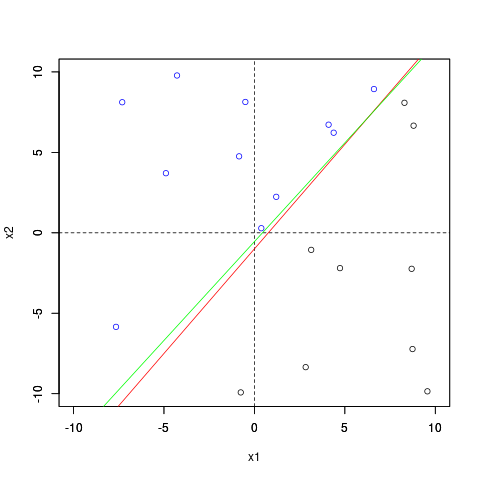
\includegraphics[scale=0.75]{figs/ex1.4_PLA.png}
		 	\caption{Red - Original Line; Green - PLA line}
		 \end{figure} 
	 
		 The process in implemented \href{https://github.com/reneroliveira/Machine_Learning/blob/main/Exercises/PLA_algorithm.R}{here}. And a result, the code returns some information to the console and generates the Figure \ref{pla}. The red line was the one used for data classification, and the green line was discovered by the PLA algorithm. Below yoy can see executon time, the line coefficients and number of iterations:
		 
		 \begin{lstlisting}[language=R]
 [1] "Execution Time: 0.0584745407104492 secs"
 [1] "Iterations: 16"
 [1] "Real Angular Coefficient -> 1.3"
 [1] "PLA Angular Coefficient -> 1.22830366623333"
 [1] "Real Linear Coefficient -> -1"
 [1] "PLA Linear Coefficient -> -0.548887922667682"
		 \end{lstlisting}
		 
		 \textbf{Exercise 1.8:}
		 
		 If $\mu=0.9$, what is the probability that a sample of $10$ marbles will have $\nu\leq 0.1$? [\emph{Hints: 1. Use binomial distribution. 2. The answer is a very small number}]
		 
		 \textit{Solution: } The context is a bin that contains red and green marbles, with $\mu$ being the unknown probability of randomly picking a red marble. $\nu$ is the proportion of red marbles in a sample with replacement.
		 
		 If $X_i$ is the random indicator variable for the $i$-th marble being red, $X_1,X_2,...,X_10$ are independent and indentically distribuited with a bernoulli($\mu$) distribution.
		 
		 The sum $S=\sum_{i=1}^{10}X_i$ is a $\operatorname{bibomial}(10,\mu)$ variable. We want to compute $\mathbb{P}(S/10\leq 0.1)=\mathbb{P}(S\leq 1)$ which is:
		 
		 \begin{align*}
		 &\displaystyle\sum_{i=0}^{1}{10 \choose i}\mu^i(1-\mu)^{n-i}\\
		 &=\mu^0(1-\mu)^{10}+45\mu(1-\mu)^9\\
		 &=(0.1)^{10}+45(0.9)(0.1)^9\\
		 &=10^{-10}(1+405)\\
		 &=4.06\times 10^{-8}
		 \end{align*}
		 
		 A very small number for sure!
		 
	\textbf{Exercise 1.9:}
	
	If $\mu=0.9$, use Hoeffding Inequality to bound the probability that a sample of 10 marbles will have $\nu\leq 0.1$ and compare the answer to the previous exercise.
	
	\textit{Solution:} 
	
	The \textit{Hoeffding Inequality}\cite{yaser2012learning} states that, for any sample size $N$,
	
	$$\mathbb{P}[|\nu-\mu|>\varepsilon]\leq2 e^{-2\varepsilon^2N},~~~\forall~\varepsilon>0$$
	
	In our case, $N=10$. and we want to bound the probability of the proportion of red marbles $\nu$ is less than $0.1$; therefore, we want no know the probability of the distante $|\nu-\mu|$ exceeds $0.8$, then we just set $\varepsilon=0.8$ and apply the formula:
	
	\begin{align*}
		\mathbb{P}[|\nu-\mu|>0.8]\leq 2 e^{-20(0.8)^2}=2e^{-12.8}\approx 5.521 \times 10^{-6}
	\end{align*}
	
	Comparing this bound with the exact probability found in the last exercise, we can see that Hoeffding's bound is around 135 times the real answer. Besides that, it is still a tiny number, making it clear that observing a 0.1 proportion (or less than that) of red marbles in a 10-marbles sample of a bin with $\mu=0.9$ is very unlikely. 
\newpage

% \addcontentsline{toc}{section}{Referências}
\bibliographystyle{plain}
\bibliography{references}
\end{document}